\documentclass[final,1p,times]{elsarticle}
\usepackage[utf8]{inputenc}

\makeatletter
\def\ps@pprintTitle{%
   \let\@oddhead\@empty
   \let\@evenhead\@empty
   \let\@oddfoot\@empty
   \let\@evenfoot\@oddfoot
}
\makeatother

\usepackage[hyphens]{url}
\usepackage{amsmath,amssymb,amsthm}
\DeclareMathOperator*{\E}{\mathbb{E}}
\DeclareMathOperator*{\F}{\mathbb{F}}
\DeclareMathOperator*{\argmin}{arg\,min}

\usepackage[normalem]{ulem}
\usepackage{fancyvrb}

\newcommand{\twovec}[2]{\left[\begin{array}{c} #1 \\ #2 \end{array}\right]}
\newcommand{\threevec}[3]{\left[\begin{array}{c} #1 \\ #2 \\ #3\end{array}\right]}

\newcommand{\drawHDsquiggle}[1]{\draw[-stealth, decoration={snake, amplitude = .4mm, segment length = 1.5mm, post length=0.9mm},decorate] (#1)+(-0.75, 0.5) -- (#1);}
\newcommand{\drawDHsquiggle}[1]{\draw[-stealth, decoration={snake, amplitude = .4mm, segment length = 1.5mm, post length=0.9mm},decorate] (#1)+(0.75, 0.5) -- (#1);}

\usepackage{tikz}
\usepackage{marvosym}
\usetikzlibrary{backgrounds}
\usetikzlibrary{decorations.pathmorphing}
\usetikzlibrary{arrows, positioning, shapes.geometric}
\tikzset{->,>=stealth',shorten >=1pt,auto,
    node distance=1cm, thick,
    bellman/.style={circle,draw},
    root/.style={circle,draw,fill,gray},
    triangle/.style={regular polygon, regular polygon sides=3,draw},
    branch/.style={diamond,draw},
    rectangle/.style={regular polygon sides=4,draw},
    square/.style={regular polygon,regular polygon sides=4,draw},
    textnode/.style={}}

\usepackage{csquotes}

\begin{document}

\begin{frontmatter}

\title{SOLIB: A Benchmark Library for Stochastic Optimization}

\author[label1]{Oscar Dowson\corref{cor1}}
\address[label1]{Department of Engineering Science at The University of Auckland, 70 Symonds Street, Auckland 1010, New Zealand}

\cortext[cor1]{Corresonding author}
\ead{odow003@aucklanduni.ac.nz}

\begin{abstract}
    The field of computational stochastic optimization is highly fragmented. In this paper we propose a graphical framework for communicating a large class of computational stochastic optimization models, and define a common file-format for representing such problems. We have collated the beginnings of a test-set of real-world models (named SOLIB - Stochastic Optimization Library) and used SOLIB to perform a comparison between to variations of the Stochastic Dual Dynamic Programming algorithm.
\end{abstract}

\begin{keyword}
multistage \sep computational stochastic optimization \sep stochastic programming
\end{keyword}

\end{frontmatter}

\section{Introduction}

In 1974, Klingman et al. \cite{klingman} wrote ``one of the problems ... in trying to benchmark codes based on different methodologies ... [is] their lack of uniformity for input specification. This nonstandardization of problem specification ... is most frustrating and has hampered benchmarking since researchers are reluctant to recode their input routines.'' In 2007, Gassmann and Kristjansson \cite{smps} highlighted this remark and compared it to the then current state of stochastic optimization. However, as far back as 1987, Birge et al. \cite{birge} wrote that efforts to solve stochastic optimization problems ``have tended to be directed towards specialized types of problems resulting in a pot-pourri of numerical codes, problem formulations and data sets that are not comparable or even mutually compatible. The development of general purpose codes suitable for industrial application is hampered by the lack of a comprehensive set of test problems in a standard format to compare performance and challenge competitors.'' The file format they laid out in \cite{birge}, now called SMPS (Stochastic Mathematical Programming System), was a format they ``hope[d] will become the nucleus of a standard problem format for multistage stochastic linear programs.''

Despite this hope, twenty years later, in 2007, Gassmann and Kristjansson wrote \cite{smps} that ``while [the SMPS format] is widely used, SMPS does not enjoy universal acceptance. Part of the reason is that the record-based structure of MPS is deemed to be overly rigid and limiting, but we feel that at least in part the reason is a lack of examples that describe the many and varied constructs of the SMPS format.''

Now, ten years later still, and thirty years after the original paper by Birge et al., a number of test-sets have been collated \cite{POSTS,slpset,siplib, wright,saphir}. While these appear to demonstrate the flexibility of the SMPS standard, we highlight a number of features that are, in our view, large short-comings. Namely, these are
\begin{enumerate}
    \item The diverging scenario-tree based approach. It is impossible\footnote{I haven't found an example or documentation to say otherwise.} for a child node to be descended from two parents. This is important in order to avoid the exponential growth in the number of leaves of the scenario tree;
    \item The reliance on the MPS standard (neither human readable, nor machine efficient);
    \item The reliance on temporal ordering of coefficients in the Core file;
    \item The lack of a clear definition of a state variable;
    \item The inability to specify non-quadratic terms. 
\end{enumerate}

Furthermore, despite the large number of test-problems, tools for reading, writing, and solving problems in the SMPS standard are not widespread. We hypothesize that the reason for this is not deficiencies in the SMPS standard, but an overall fragmentation of the community in general.

In recent years, Powell \cite{powell_jungle,powell_tutORial} has highlighted the fragmentation of our field, and made the case for unifying the various communities of Stochastic Optimization (which goes by various names including Optimal Control, Stochastic Search, Dynamic Programming, Robust Optimization, etc.) under the umbrella of \emph{Computational Stochastic Optimization} (henceforth referred to as CSO). Indeed, for terms as widely used as \emph{state} and \emph{stage}, there seems to be no widely agreed upon definition.\footnote{See Powell's comment in \cite{powell_jungle} ``there is an astonishing lack of agreement in the definition of a state variable.''} This makes it hard to develop standards and share work when we cannot even agree what it is that we are trying to share.

Another reason for the limited uptake may be the lack of an open-source, unified set of modelling languages and solution algorithms in modern computational languages (e.g. Julia, Python). Consider the problem of solving a dynamic program (not even necessarily stochastic) via backwards recursion. The practitioner must re-invent the wheel, and usually codes such an implementation in a low-level language such as C or C++ to get performance. They usually seek the path of least resistance and implement the bare-minimum required to solve a particular problem or prove a particular algorithm's performance. They are unlikely to go to the effort of implementing an SMPS reader (let alone writer), and therefore find no incentive to copy their new models across to a standard they don't support.

SMPS is not the only file-format that has been proposed to stochastic optimization problems. Another competing file-format that can be used to represent stochastic optimization problems is the OSiL (Optimization Services instance Language) file-format \cite{fourer_xml-based_2009}. OSiL uses an XML based schema for representing problem data. This means the file is more human readable (and editable) than the SMPS files. In addition, it is able to specify arbitrary non-linear terms by creating a nested expression graph. Unlike the SMPS format, the OSiL format has a number of different ways of specifying the uncertainty. These include explicit scenario trees (like the SMPS format), as well as implicit scenario trees by describing the different random variables at each stage. However, OSiL makes the same error as the SMPS format, in that, despite decomposing the problem into \emph{stages}, and identifying random variables and non-anticipativity constraints, it fails to clearly identify state variables in the canonical form it can support. In our view, this leads to a format that is more complicated than necessary.

We echo the words of Birge et al., and believe that the CSO community has been held back by this fragmentation. Therefore, we propose four goals which should be given top priority by the community:

\begin{enumerate}
    \item The standardization of definitions and problem specifications from a mathematical standpoint;
    \item The creation, and adoption, of a common file-format for sharing CSO problems;
    \item The maintenance of an archive of CSO problems in that file-format;
    \item The development of a suite of inter-operable, open-source modeling libraries and solvers for CSO.
\end{enumerate}

In this paper we attack the first three points. We refer the reader to (TODO \texttt{SDDP.jl} paper) for a discussion of some recent advancements in respect to the fourth point. In section \ref{sec:staging}, we discuss the staging of computational stochastic optimization problems (namely the question: what is a stage?) and present the idea of a \emph{stage graph}. In section \ref{sec:canonical}, we outline the canonical form we use to represent CSO problems that arises naturally from the concept of a stage graph. Lastly, in section \ref{sec:fileformat}, we propose a new file-format for a sub-class of CSO problems (those with discrete random variables with known probabilities) that is a close representation of the canonical form from section \ref{sec:canonical}. This new file-format overcomes many of the limitations identified in the SMPS and OSiL file-formats, and clearly identifies the decomposition structure of the problem.

\section{Staging of CSO problems}\label{sec:staging}

In \cite{powell_jungle}, Powell makes the case that almost all stochastic optimization problems can be formulated as a sequential decision problem with an exogenous, memoryless (markovian), information process. For this paper we ignore continuous time problems and only consider problems where the sequential decision making happens in discrete time. Continuous time problems have been extensively studied and can be more easily described by partial differential equations, rather than the approach we advocate in this paper.

Powell identifies the five dimensions of any stochastic optimization problem as:
\begin{enumerate}
    \item State variables: We take the definition from \cite{powell_tutORial} as:

\emph{The state variable is the minimally dimensioned function of history that captures all the information we need to model a system from some point in time onward.}

These state variables can be continuous or discrete. We denote them with the lowercase $x_t$ at time $t$.

    \item Control variables: A control variable is an action or decision taken by the operator (whether explicitly or implicitly) that changes the state of the system.
    
    These can be continuous or discrete. We denote them with the lowercase $u_t$ at time $t$.
    
    \item Exogenous information (the uncertainty). A noise is a (potentially multi-dimensional) random variable that is exogenous to the state of the system and the controls chosen by the operator. We denote a single observation of the random variable with the lowercase $\omega_t$ and the distribution from which it is drawn by the uppercase $\Omega_t$ at time $t$.
    
    \item Transition function: the transition function is a (potentially unknown) mapping of the current state $x_t$, the control $u_t$ and a realization of the noise $\omega_t$ to a new state $x'_t$.
    
    \item Objective function: the cost (reward) accrued by taking action $u_t$ in state $x_t$ and realization $\omega_t$.
\end{enumerate}

We believe this list is missing one important item: an explicit representation of the sequential ordering of the decision making (in other words, how the exogenous information is revealed over the decision making process). In theory, this information is implicit within the five dimensions, however as we shall see, there are clear benefits from making the staging process explicit.

The core decomposition feature of a computational stochastic optimization problem is the stage. There are two types of stages:

\paragraph{1. Hazard-Decision} In a Hazard-Decision stage (Figure \ref{fig:d}), the operator chooses an action $u_i$ after observing a realization of the random variable $\omega_i \sim \Omega_i$ according to a policy $\pi_i(x_i, \omega_i)$. The state transitions from $x_i$ to $x_{i+1}$ according to the transition function $T_i(x_i, u_i, \omega_i)$. The policy respects the set of admissible actions so that $u_i\in U_i(x_i, \omega_i)$ and $x_{i+1}\in \mathcal{X}_i$. In addition, a cost $C_i(x_i, u_i, \omega_i)$ is incurred.

\begin{figure}[!ht]
    \centering
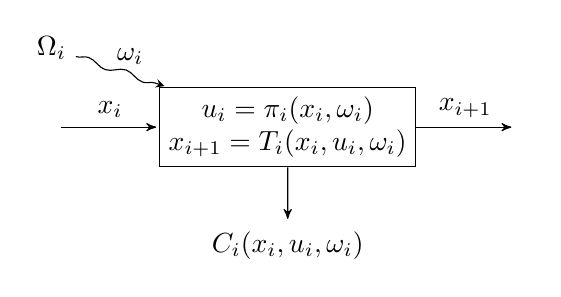
\begin{tikzpicture}
[align=center,node distance=3cm]
\node[textnode] (a)  [] {};
\node[rectangle] (b)  [right of = a] {$u_i=\pi_{i}(x_i, \omega_i)$\\$x_{i+1} = T_i(x_i, u_i, \omega_i)$};

\node[textnode] (w) at (0,1) {$\Omega_i$};
\node[textnode] (cst)  at (3, -1.5) {$C_i(x_i, u_i, \omega_i)$};

\node[textnode] (c)  [right of = b] {};
\path[]
	(a)	edge 	[] 	node	[left] 	[above] {$x_i$}	(b)
	(b)	edge 	[] 	node	[left] 	[above] {}	(cst)
% 	(w)	edge 	[] 	node	[left] 	[above] {$\omega_i$}	(b)
    (b)	edge 	[] 	node	[left] 	[above] {$x_{i+1}$}	(c);
    
\draw[-stealth, decoration={snake, amplitude = .4mm, segment length = 5mm, post length=0.9mm},decorate] (w) -- (b);

\node [align=center] (ww) at (1,0.9) {$\omega_i$};
\end{tikzpicture}
\caption{Hazard-Decision stage.}
\label{fig:d}
\end{figure}

\paragraph{2. Decision-Hazard} In a Decision-Hazard stage (Figure \ref{fig:dh}), the operator chooses an action $u_i$ before observing a realization of the random variable $\omega_i \sim \Omega_i$ according to a policy $\pi_i(x_i)$. The state transitions from $x_i$ to $x_{i+1}$ according to the transition function $T_i(x_i, u_i, \omega_i)$. The policy respects the set of admissible actions so that $u_i\in U_i(x_i)$ and $x_{i+1}\in \mathcal{X}_i$. In addition, a cost $C_i(x_i, u_i, \omega_i)$ is incurred.

\begin{figure}[!ht]
    \centering
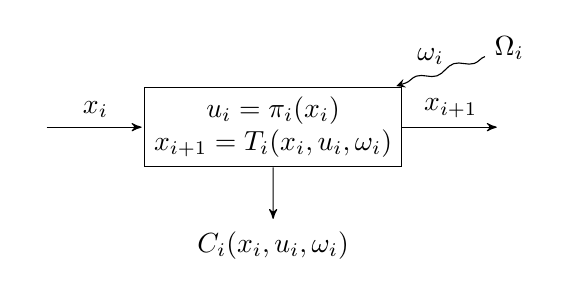
\begin{tikzpicture}
[align=center,node distance=3cm]
\node[textnode] (a)  [] {};
\node[rectangle] (b)  [right of = a] {$u_i=\pi_{i}(x_i)$\\$x_{i+1} = T_i(x_i, u_i, \omega_i)$};

\node[textnode] (w) at (6,1) {$\Omega_i$};
\node[textnode] (cst)  at (3, -1.5) {$C_i(x_i, u_i, \omega_i)$};

\node[textnode] (c)  [right of = b] {};
\path[]
	(a)	edge 	[] 	node	[left] 	[above] {$x_i$}	(b)
	(b)	edge 	[] 	node	[left] 	[above] {}	(cst)
    (b)	edge 	[] 	node	[left] 	[above] {$x_{i+1}$}	(c);
\draw[-stealth, decoration={snake, amplitude = .4mm, segment length = 5mm, post length=0.9mm},decorate] (w) -- (b);
\node [align=center] (ww) at (5,0.9) {$\omega_i$};
\end{tikzpicture}
\caption{Decision-Hazard stage.}
\label{fig:dh}
\end{figure}

When there is no uncertainty that is realized in the stage, the Decision-Hazard stage becomes identical to the Hazard-Decision stage. We denote this deterministic stage by dropping the wavy line coming into the stage.

\subsection{Stage Graph}

CSO problems usually involve more than one stage chained in sequence. In this section we show by example a graph based approach to defining multi-stage problems that is able to describe any combination of sequential decision making processes. Shaded gray circles are the root nodes. A root node contains the initial value of the state variables, and is typically the point in the decision making process that we calculate the objective of the optimization problem.

% Dashed grey ellipses are used to isolate the different stage problems. 

We call the graph describing the stages the \emph{stage graph}. For simplicity, we drop the textual annotations used above as their values can be inferred based on the type of symbol used.

\paragraph{Deterministic Sequential Decision problem}

In the deterministic setting, the system is in a given state, and action is then chosen that transitions the system to a new state (Figure \ref{fig:det}).

\begin{figure}[!ht]
    \centering
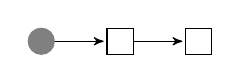
\begin{tikzpicture}
\node[root] (a)  []              {};
\node[square] (b)  [right of = a]              {};
\node[square] (c)  [right of = b]              {};
\path[]
	(a)	edge 	[] 	node	[left] 	{}	(b)
    (b)	edge 	[] 	node	[left] 	{}	(c);
\end{tikzpicture}
\caption{Two-stage Decision-Only problem.}
\label{fig:det}
\end{figure}

\paragraph{Sequential Hazard-Decision problem}

In a sequential Hazard-Decision problem (Figure \ref{fig:shd}), the noise is observed before the action is taken.

\begin{figure}[!ht]
    \centering
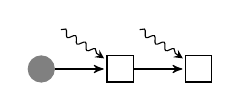
\begin{tikzpicture}
\node[root] (a)  []              {};
\node[square] (b)  [right of = a]              {};
\node[square] (c)  [right of = b]              {};
\path[]
	(a)	edge 	[] 	node	[left] 	{}	(b)
    (b)	edge 	[] 	node	[left] 	{}	(c);

\drawHDsquiggle{b}
\drawHDsquiggle{c}
\end{tikzpicture}
\caption{Two-stage Hazard-Decision problem.}
\label{fig:shd}
\end{figure}

A stage graph can also be thought of as a compressed scenario tree. It is also possible to express the problem as an explicit scenario tree. If each Hazard-Decision stage in Figure \ref{fig:shd} has two possible realizations for $\omega$, the scenario tree has six Decision-Only stages (Figure \ref{fig:scenario}). The uncertainty lies on the exiting arcs from the stage problems.

\begin{figure}[!ht]
    \centering
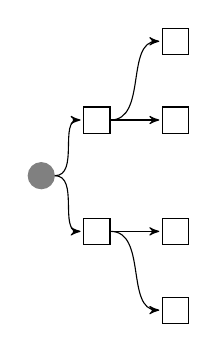
\begin{tikzpicture}
\node[root]    (a)  []                   {};
\node[square]  (b)  [below right of = a] {};
\node[square]  (c)  [above right of = a] {};
\node[square]  (d)  [right of = b]       {};
\node[square]  (e)  [below of = d]       {};
\node[square]  (f)  [right of = c]       {};
\node[square]  (g)  [above of = f]       {};

\path[out=0,in=180]
    (a)	edge 	[] 	node	[left] 	{}	(b)
    (a)	edge 	[] 	node	[left] 	{}	(c)
    (b)	edge 	[] 	node	[left] 	{}	(d)
    (b)	edge 	[] 	node	[left] 	{}	(e)
    (c)	edge 	[] 	node	[left] 	{}	(f)
    (c)	edge 	[] 	node	[left] 	{}	(g);
\end{tikzpicture}
\caption{Explicit scenario-tree representation.}
\label{fig:scenario}
\end{figure}

Any stage graph (with finite, discrete, distributions for $\Omega$) can be expanded into a scenario tree, but a scenario tree cannot be compressed into a stage graph without information about which branches are independent.

\paragraph{Sequential Decision-Hazard problem}

In a sequential Decision-Hazard problem (Figure \ref{fig:sdh}), the noise is observed after the action is chosen. 

\begin{figure}[!ht]
    \centering
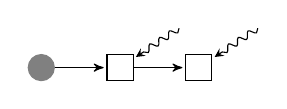
\begin{tikzpicture}
\node[root]     (a)  []              {};
\node[square]   (b)  [right of = a]              {};
\node[square]   (c)  [right of = b]              {};

\path[]
	(a)	edge 	[] 	node	[left] 	{}	(b)
    (b)	edge 	[] 	node	[left] 	{}	(c);

\drawDHsquiggle{b}
\drawDHsquiggle{c}
\end{tikzpicture}
\caption{Staged Here-and-Now (Decision-Hazard) Problem.}
\label{fig:sdh}
\end{figure}

\paragraph{Two-stage with recourse}

A common problem in the literature is the two-stage problem with recourse (Figure \ref{fig:2stage}). In this problem, the operator chooses a first stage decision $u_1$, realizes some uncertainty, and then can take a recourse decision based on the observation of the uncertainty.

\begin{figure}[!ht]
    \centering
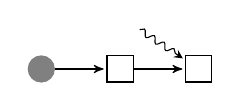
\begin{tikzpicture}
\node[root]   (a)  []              {};
\node[square] (b)  [right of = a]              {};
\node[square] (c)  [right of = b]              {};
\path[]
	(a)	edge 	[] 	node	[left] 	{}	(b)
    (b)	edge 	[] 	node	[left] 	{}	(c);
\drawHDsquiggle{c}
\end{tikzpicture}
\caption{Two-stage recourse problem.}
\label{fig:2stage}
\end{figure}

\subsubsection{Conditional-Dependence}\label{sec:conditional}

In this section we depart slightly from Powell's claim that all properly modeled systems are markovian. It can be the case that when a state variable depends \emph{only} on the exogenous information process (and not on the rest of the state variables, or the control variables), then it is possible to combine both a markovian information process and a discrete scenario tree.

For a motivating example for Figure \ref{fig:conditional}, consider the following: The El Ni\~no-Southern Oscillation is a irregular, periodical climate pattern in the Pacific Ocean. It has two extremes: El Ni\~no and La Ni\~na. In El Ni\~no years, the Eastern Pacific warms relative to average, and there is less rainfall than average in the Western Pacific. In La Ni\~na years, the opposite is true. When the first decision is taken, it is unknown whether the year will be El Ni\~no or La Ni\~na. Once this is revealed, a recourse decision can be taken, before the actual rainfall is observed. 

We could model this as a single branch, two-stage problem like Figure \ref{fig:2stage}, but we would need to encode an additional state variable (the belief about whether the system was in El Ni\~no or La Ni\~na).

To model conditional-dependence in the information process, we allow multiple arcs to exit from a stage. Each arc is associated with a probability such that the sum of the probabilities on the arcs leaving a stage sums to one. In addition, multiple arcs can enter a stage.

% \begin{figure}[!ht]
%     \centering
% \begin{tikzpicture}
% \node[root]  (a)  []              {\$};
% \node[square]   (b)  [right of = a]              {};
% \node[bellman]  (bb)  [right of = b]              {\$};

% \node[branch] (c)  [right of = bb]              {};

% \node[triangle] (d)  [below right of = c]              {};
% \node[square]   (e)  [right of = d]              {};
% \node[bellman]  (f)  [right of = e]              {\$};
% \node[triangle] (g)  [above right of = c]              {};
% \node[square]   (h)  [right of = g]              {};
% \node[bellman]  (i)  [right of = h]              {\$};
% \path[]
% 	(a)	edge 	[] 	node	[left] 	{}	(b)
%     (b)	edge 	[] 	node	[left] 	{}	(bb)
%     (bb)	edge 	[] 	node	[left] 	{}	(c)
%     (c)	edge 	[] 	node	[left] 	{}	(d)
%     (d)	edge 	[] 	node	[left] 	{}	(e)
%     (e)	edge 	[] 	node	[left] 	{}	(f)
%     (c)	edge 	[] 	node	[left] 	{}	(g)
%     (g)	edge 	[] 	node	[left] 	{}	(h)
%     (h)	edge 	[] 	node	[left] 	{}	(i);
    
% \begin{pgfonlayer}{background}
% \draw [gray,thick, dashed] (1.45,0) ellipse (0.9cm and 0.6cm);
% \draw [gray,thick, dashed] (4.6,0.7) ellipse (1.45cm and 0.6cm);
% \draw [gray,thick, dashed] (4.6,-0.7) ellipse (1.45cm and 0.6cm);
% \end{pgfonlayer}

% \end{tikzpicture}
% \caption{Two-stage recourse problem with conditional dependence.}
% \label{fig:conditional}
% \end{figure}
% \begin{figure}[!ht]
%     \centering
% \begin{tikzpicture}
% [align=center,node distance=2.5cm]
% \node[root]   (a)  []              {};
% \node[square] (b)  [right of = a] {$\pi_1(x_0)$};
% \node[inner sep=0,minimum size=0,right of=b] (k) {}; % invisible node
% \node[branch] (c)  [above right of = k] {$\pi_2(x_1, \omega_2)$};
% \node[branch] (d)  [below right of = k] {$\pi_3(x_1, \omega_3)$};
% \path[]
% 	(a)	edge 	[] 	node	[above] 	{$x_0$}	(b)
% 	(b)	edge 	[] 	node	[above] 	{$x_1$}	(k)
%     (k)	edge 	[] 	node	[above,rotate=45] 	{w.p. 0.5}	(c)
%     (k)	edge 	[] 	node	[below,rotate=-45] 	{w.p. 0.5}	(d);
% \end{tikzpicture}
% \caption{Two-stage recourse problem with conditional dependence.}
% \label{fig:conditional}
% \end{figure}

\begin{figure}[!ht]
    \centering
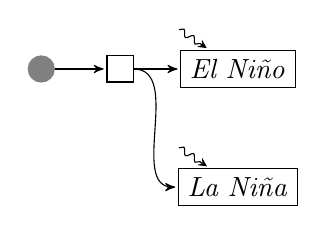
\begin{tikzpicture}
% [align=center,node distance=2.5cm]
\node[root]   (a)  []              {};
\node[square] (b)  [right of = a] {};
\node[rectangle,node distance=1.5cm] (c)  [right of = b] {\textit{El Ni\~no}};
\node[rectangle,node distance=1.5cm] (d)  [below of = c] {\textit{La Ni\~na}};
\path[out=0,in=180]
	(a)	edge (b)
	(b)	edge (c)
	(b)	edge (d);
\drawHDsquiggle{c}
\drawHDsquiggle{d}
\end{tikzpicture}
\caption{Two-stage recourse problem with conditional dependence.}
\label{fig:conditional}
\end{figure}

It is also possible for the conditional-dependence to be markovian (Figure \ref{fig:markovian}). This recombination of the scenario tree helps prevent the number of leaf nodes from growing exponentially.

\begin{figure}[!ht]
    \centering
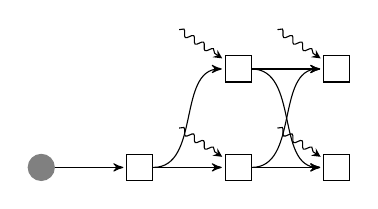
\begin{tikzpicture}
[align=center,node distance=1.25cm]
\node[root]   (a)  []              {};
\node[square] (b)  [right of = a] {};
\node[square] (c)  [right of = b] {};
\node[square] (d)  [above of = c] {};
\node[square] (e)  [right of = c] {};
\node[square] (f)  [above of = e] {};
\path[out=0,in=180]
	(a)	edge 	[] 	node	[above] 	{}	(b)
    (b)	edge 	[] 	node	[] 	{}	(c)
    (b)	edge 	[] 	node	[] 	{}	(d)
    (c)	edge 	[] 	node	[] 	{}	(e)
    (c)	edge 	[] 	node	[] 	{}	(f)
    (d)	edge 	[] 	node	[] 	{}	(e)
    (d)	edge 	[] 	node	[] 	{}	(f);
\drawHDsquiggle{c}
\drawHDsquiggle{d}
\drawHDsquiggle{e}
\drawHDsquiggle{f}
\end{tikzpicture}
\caption{Multi-stage recourse problem with markovian conditional dependence.}
\label{fig:markovian}
\end{figure}

Another reason for introducing a scenario tree is an example like Figure \ref{fig:multi}. In one branch of the tree, there are two sequential decisions, in the other, there are three. One way to consider this problem is that there are three sequential decisions in all branches, and that the feasible action space of the third decision on the lower branch is the null set. Furthermore, some stages are deterministic, some are Decision-Hazard, and some are Hazard-Decision.

\begin{figure}[!ht]
    \centering
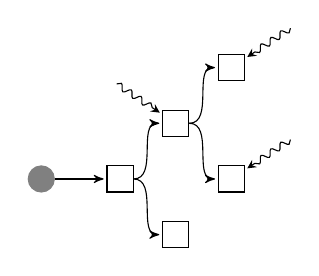
\begin{tikzpicture}
% [align=center,node distance=2.5cm]
\node[root]   (a)  []              {};
\node[square] (b)  [right of = a] {};
\node[square] (c)  [above right of = b] {};
\node[square] (d)  [below right of = b] {};
\node[square] (e)  [above right of = c] {};
\node[square] (f)  [below right of = c] {};
\path[out=0,in=180]
	(a)	edge 	[] 	node	[above] 	{}	(b)
    (b)	edge 	[] 	node	[] 	{}	(c)
    (b)	edge 	[] 	node	[] 	{}	(d)
    (c)	edge 	[] 	node	[] 	{}	(e)
    (c)	edge 	[] 	node	[] 	{}	(f);
\drawHDsquiggle{c}
\drawDHsquiggle{e}
\drawDHsquiggle{f}
\end{tikzpicture}
\caption{Multi-stage recourse problem conditional dependence.}
\label{fig:multi}
\end{figure}

\subsubsection{Cyclic Graphs}

It is also possible to capture Infinite Horizon problems with the graph based approach (Figure \ref{fig:cycle}. These can be feedback loops (for example, from stochastic optimal control), or even sub-graphs embedded inside a larger graph (Figure \ref{fig:extcycle}).

\begin{figure}[!ht]
    \centering
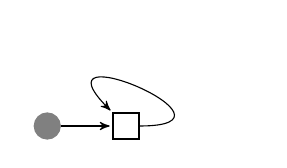
\begin{tikzpicture}
\node[root]    (a)  []              {};
\node[square]  (b) [right of=a]  {};
\draw (b) to [out=0,in=135,looseness=10] (b);
\path[]
	(a)	edge 	[] 	node [] {} (b);
\end{tikzpicture}
\caption{Infinite Horizon Problem.}
\label{fig:cycle}
\end{figure}

\begin{figure}[!ht]
    \centering
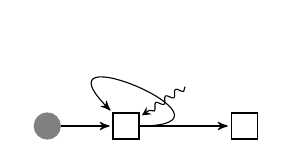
\begin{tikzpicture}
\node[root]    (a)  []              {};
\node[square]  (b) [right of=a]  {};
\node[square,node distance=1.5cm]  (c) [right of=b]  {};
\draw (b) to [out=0,in=135,looseness=10] (b);
\path[]
	(a)	edge 	[] 	node [] {} (b)
	(b)	edge 	[] 	node [] {} (c);
\drawDHsquiggle{b}
\end{tikzpicture}
\caption{Infinite Horizon Problem.}
\label{fig:extcycle}
\end{figure}

Typically, these involve the need to add a \emph{discount factor} in order to discount the future costs. The question arises how to incorporate these into the \emph{stage graph}. The solution we propose, it to allow the probabilities of the arcs exiting a bellman node to sum to less than one. Implicitly, this results in the addition of an additional leaf stage with zero cost (Figure \ref{fig:discount}). The \emph{discount factor} $\lambda$ can be interpreted as a 1 - probability that the system stops. 

\begin{figure}[!ht]
    \centering
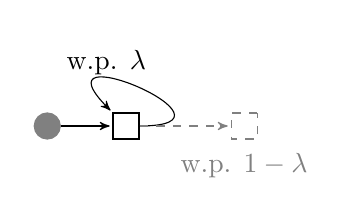
\begin{tikzpicture}
\node[root]    (a)  []              {};
\node[square]  (b) [right of=a]  {};
\node[square,node distance=1.5cm, dashed, gray]  (c) [right of=b]  {};
\draw (b) to [out=0,in=135,looseness=10] (b);
\path[]
	(a)	edge 	[] 	node [] {} (b)
	(b)	edge 	[dashed, gray] 	node []{} (c);

\node[] (discount) at (0.75,0.8) {w.p. $\lambda$};	
\node[gray] (lambda) at (2.5,-0.5) {w.p. $1-\lambda$};
	
% \node[root]   (a) {};
% \node[square, right of=a] (b) {};
% \node[inner sep=0,minimum size=0,right of=b] (k) {}; % invisible node
% \node[inner sep=0,minimum size=0,right of=k] (j) {}; % invisible node
% \node[inner sep=0,minimum size=0,right of=j] (l) {w.p. $1-\lambda$}; % invisible node
% % \node[branch]  (c) [right of=k]  {};
% % \draw (k) to [] (b) [below] {w.p. $\lambda$};
% \path[]
% 	(a)	edge 	[] 	node [] {} (b)
% 	(b)	edge 	[] 	node [] {} (k)
% 	(k)	edge 	[out=45,in=135,looseness=3] 	node [above] {w.p. $\lambda$} (b)
% 	(k)	edge 	[] 	node [below] {} (j);
\end{tikzpicture}
\caption{Cyclic graph with explicit discount.}
\label{fig:discount}
\end{figure}


\section{Canonical form of a CSO Problem}\label{sec:canonical}

In \cite{powell_tutORial}, Powell proposed the canonical form for a CSO problem as

\begin{equation}
    \max\limits_\pi \E \left\{\sum\limits_{t=0}^T C(S_t, X_t^\pi(S_t))\ |\ S_0 \right\},
    \label{eq:powellcanonical}
\end{equation}

where decisions are made according to a policy $x_t=X_t^\pi(S_t)$, where we might use $a_t =A_t^\pi(S_t)$ for discrete actions, or $u_t=U_t^\pi(x_t)$ for state $x_t$ and control $u_t$. States evolve according to a (possibly unknown) transition function $S_{t+1}=S^M(S_t,X_t^\pi(S_t),W_{t+1})$.

This desire for a compact canonical form is admirable (it is hard to beat $min\left\{c^\top x\ |\ Ax = b\right\}$), but it unnecessarily obscures details about the staging of a CSO problem (it is also unclear how to deal with nested risk-measures). We prefer the recursive definition of (\ref{eq:powellcanonical}) for CSO problems:

\begin{equation}
    \min\limits_\pi \F\limits_{i\in0^+;\ \omega \in \Omega_i}\left[V^\pi_i(x_0, \omega) \right]\ |\ x_0,
\end{equation}

where

\begin{equation}
  V^\pi_i(x_i, \omega) = C_i(x_i, u_{i,\omega}, \omega) + \F\limits_{j\in i^{+},\  \omega_j \in \Omega_j} \left[V^\pi_j(x_{i,\omega}, \omega_j)\right],
\end{equation}

$x_{i,\omega} = T_i(x_i, u_{i,\omega}, \omega)$. If the stage $i$ is Hazard-Decision $u_{i,\omega} = \pi_i(x_i, \omega)$, otherwise the stage is Decision-Hazard and $u_{i,\omega} = \pi_i(x_i)$. The policy respects any constraints on the domain of the control so that $u_{i,\omega} \in U_i(x_i, \omega)$ if the stage is Hazard-Decision and $u_{i,\omega} \in U_i(x_i)$ if the stage is Decision-Hazard. $\F$ is a risk measure. $i^+$ is the set of child nodes of stage $i$. There is a known, finite probability of transitioning from stage $i$ to every stage in $i^+$. The set of nodes $0^+$ are the children of the root node. We also assume relatively complete recourse of $x_i$. That is, for all $\omega \in \Omega_i$ and possible incoming values of $x_i$, there is a feasible control $u_{i,\omega}$, with a bounded objective value $V^\pi_i(x_i,\omega)$.

In the stochastic optimization community, Hazard-Decision policies are typically constructed by forming a mathematical optimization problem. Therefore, $V^\pi_i(x_i, \omega)$ is the objective of the optimization problem:

\begin{equation}
\begin{array}{l r l}

    \textbf{HD}_i(x_i, \omega):\quad & \min\limits_{u_{i,\omega}}& C_i(x_i, u_{i,\omega}, \omega) + \F\limits_{j\in i^{+};\ \varphi\in\Omega_j} \left[V^\pi_j(x_{i,\omega}, \varphi)\right] \\
   &{s.t.} & x_{i,\omega} = T_i(x_i, u_{i,\omega}, \omega)\\
   &       & u_{i,\omega} \in U_i(x_i, \omega),
\end{array}
\label{eq:stageproblem}
\end{equation}

and the policy $\pi_i(x_i, \omega) \in \argmin\limits_{u_{i,\omega}} \textbf{HD}_i(x_i, \omega)$. The future cost component of the objective is usually non-trivial, and so approximation schemes are used.

A Decision-Hazard policy can also be formed as the optimization problem:

\begin{equation}
\begin{array}{l r l}
    \textbf{DH}_i(x_i):\quad & \min\limits_{u_i}& \F\limits_{\omega\in\Omega_i}\left[C_i(x_i, u_{i,\omega}, \omega) + \F\limits_{j\in i^{+};\ \varphi\in\Omega_j} \left[V^\pi_j(x_{i,\omega}, \varphi)\right]\right] \\
   &{s.t.} & x_{i,\omega} = T_i(x_i, u_{i,\omega}, \omega)\\
   &       & u_{i} \in U_i(x_i)\\
   &       & \underbrace{u_{i} = u_{i,\omega_1} = \dots = u_{i,\omega_N}}_{\text{Non-anticipativitiy constraint}},
\end{array}
\label{eq:detequiv}
\end{equation}

where the policy $\pi_i(x_i) \in \argmin\limits_{u_{i}} \textbf{DH}_i(x_i)$, and $V^\pi_i(x_i, \omega) = C_i(x_i, u_{i,\omega}, \omega) + \F\limits_{j\in i^{+};\ \varphi\in\Omega_j} \left[V^\pi_j(x_{i,\omega}, \varphi)\right]$. 

Equation (\ref{eq:detequiv}) can also be expressed as the two-stage stochastic program:
\begin{equation}
\begin{array}{l r l}
    \textbf{DH}_i(x_i):\quad & \min\limits_{u_i}& \F\limits_{\omega\in\Omega_i}\left[ Q_i(x_i, u_i, \omega)\right]\\
  &{s.t.} & u_{i} \in U_i(x_i),
\end{array}
\end{equation}
where $Q_i(x_i, u_i, \omega)$ is the optimal second-stage objective value of
\begin{equation}
\begin{array}{l r l}
    Q_i(x_i, u_i, \omega) =  & \min\limits_{x_{i,\omega}}& C_i(x_i, u_{i}, \omega) + \F\limits_{j\in i^{+};\ \varphi\in\Omega_j} \left[V^\pi_j(x_{i,\omega}, \varphi)\right]\\
  &{s.t.} & x_{i,\omega} = T_i(x_i, u_{i}, \omega).
\end{array}
% \label{eq:stageproblem}
\end{equation}

\subsection{Asset Management Example}\label{sec:asset}
We now give the formulation of the Asset Management problem from \cite{birgestoch} as a CSO problem. Since the transition and objective functions are linear for each of the stages, we can write the stage problems using the notation of Linear Programming.

\paragraph{Note:} by giving the stage graph transition matrix, and the distributions of $\Omega$, we don't need to include the future cost terms in the stage definition as these are implied. Therefore, we only include the $C_i(x_i,u_i,\omega)$ term in the objective.

\paragraph{Stage Graph} There are four sequential stages: \texttt{Today}; \texttt{Year 5}; \texttt{Year 10}; and \texttt{Horizon}. \texttt{Today} is a deterministic Decision-Only stage. The next three stages are Hazard-Decision problems. All arcs have probability one.

\begin{equation}
    P_{i,j} = \begin{array}{c | c c c c c}
            & \text{Today} & \text{Year 5} & \text{Year 10} & \text{Horizon}\\
            \hline
        \text{Root} & 1 & 0 & 0 & 0 \\
        \text{Today} & 0 & 1 & 0 & 0 \\
        \text{Year 5} & 0 & 0 & 1 & 0 \\
        \text{Year 10} & 0 & 0 & 0 & 1 \\
        \text{Horizon} & 0 & 0 & 0 & 0
    \end{array}
\end{equation}

\begin{figure}[!ht]
    \centering
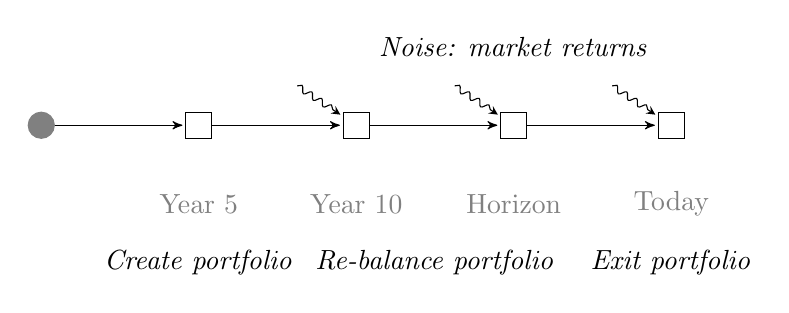
\begin{tikzpicture}
[align=center,node distance=2cm]
\node[root]   (a)  []              {};
\node[square] (b)  [right of = a]              {};
\node[square] (c)  [right of = b]              {};
\node[square] (d)  [right of = c]              {};
\node[square] (e)  [right of = d]              {};
\node[textnode, gray] (m) at (2,-1) {Year 5};
\node[textnode, gray] (n) at (4,-1) {Year 10};
\node[textnode, gray] (o) at (6,-1) {Horizon};
\node[textnode, gray] (p) at (8,-1) {Today};
\drawHDsquiggle{c}
\drawHDsquiggle{d}
\drawHDsquiggle{e}
\node [align=center] (mr) at (6,1) {\textit{Noise: market returns}};

\node [] (initial_u) at (2,-1.75) {\textit{Create portfolio}};
\node [] (y5) at (5, -1.75) {\textit{Re-balance portfolio}};
\node [] (final_u) at (8,-1.75) {\textit{Exit portfolio}};


\path[]
	(a)	edge 	[] 	node	[left] 	{}	(b)
    (b)	edge 	[] 	node	[left] 	{}	(c)
    (c)	edge 	[] 	node	[left] 	{}	(d)
    (d)	edge 	[] 	node	[left] 	{}	(e);
\end{tikzpicture}
\caption{Asset Management Structure: graph}
\end{figure}

\paragraph{Today (Decision-Only)}
\begin{equation}
    \begin{array}{l r l}
        \text{\textbf{D}}_{\text{today}}\left(\twovec{\bar{x}^s}{\bar{x}^b}\right): & \min & 0 \\
        & \text{s.t.} & x^s + x^b  = 55 + \bar{x}^s + \bar{x}^b \\
        & & x^s, x^b \ge 0,
    \end{array}
\end{equation}
where $\bar{x}^s$ is the value of stocks (in dollars) held at the start of the stage, $x^s$ is the value of stocks (in dollars) held at the end of the stage, $\bar{x}^b$ is the value of bonds (in dollars) held at the start of the stage, and $x^b$ is the value of bonds (in dollars) held at the end of the stage. The control variables (value of stocks and bonds to buy) are implicit in this formulation.

The first stage has the initial solution $(\bar{x}^s, \bar{x}^b) = (0,0)$. 

\paragraph{Year 5 and Year 10 (Hazard-Decision)}
\begin{equation}
    \begin{array}{l r l}
        \text{\textbf{HD}}_{\text{rebalance}}\left(\twovec{\bar{x}^s}{\bar{x}^b}, \twovec{\omega^s}{\omega^b}\right): & \min\limits_{\Delta} & 0 \\
        & \text{s.t.} & \omega^s\bar{x}^s + \omega^b\bar{x}^b = x^s + x^b \\
         & & x^s = \bar{x}^s + \Delta\\
        & & x^s, x^b \ge 0,
    \end{array}
\end{equation}
where $\omega^s$ is the increase in the value of the stocks during the stage, and $\omega^b$ is the increase in the value of the bonds during the stage. The control variable $\Delta$ is the value of stocks to buy.

If these stages were Decision-Hazard, we could add the constraint that $\Delta$ is non-anticipative. 

\paragraph{Horizon (Hazard-Decision)}
\begin{equation}
    \begin{array}{l r l}
        \text{\textbf{HD}}_{\text{horizon}}\left(\twovec{\bar{x}^s}{\bar{x}^b}, \twovec{\omega^s}{\omega^b}\right): & \min & 4 u - v \\
        & \text{s.t.} & \omega^s\bar{x}^s + \omega^b\bar{x}^b + u - v = 80 \\
                & & u, v \ge 0,
    \end{array}
\end{equation}
where $u$ is the quantity by which the portfolio is less than the target (\$80), and $v$ is the quantity by which the portfolio exceeds the target.

\paragraph{Exogenous Information} Stages Year 5, Year 10, and Horizon have the following probability set for $\omega$ of:

\begin{equation}
    (\omega^s, \omega^b) = \begin{cases} 
      (-1.25, -1.14) & w.p.\ 0.5, \\
      (-1.06, -1.12) & w.p.\ 0.5.
   \end{cases}
\end{equation}

%
%   I began this hoping to write the Tiger example as a CSO, but I got stuck
%   trying to figure out how to partition the state space so that the agent
%   can't use all the information, but the system can.
%
% \subsection{Tiger Example}

% To show the the canonical CSO format is not limited to stochastic optimization problems, we consider the Tiger problem from Partially Observable Markov Decision Process (POMDP) literature.

% \begin{displayquote}
% Imagine an agent standing in front of two closed doors. Behind one of the doors is a tiger
% and behind the other is a large reward. If the agent opens the door with the tiger, then a
% large penalty is received (presumably  in the form of some amount of bodily injury). Instead
% of opening one of the two doors, the agent can listen, in order to gain some information
% about the location of the tiger. Unfortunately,  listening  is not free; in addition, it is also
% not entirely accurate. There is a chance that the agent will hear a tiger behind the left-hand
% door when the tiger is really behind the right-hand  door, and vice versa.
% We refer to the state of the world when the tiger is on the left as $s_l$ and when it is on the
% right as $s_r$. The actions are  $LEFT$, $RIGHT$,  and  $LISTEN$.  The reward for opening the correct
% door is +10 and the penalty for choosing the door with the tiger behind it is -100.  The
% cost of listening  is -1. There are only two possible observations:  to hear the tiger on the
% left  ($TL$)  or to hear the tiger on the right  ($TR$).  Immediately  after the agent opens a door and
% receives a reward or penalty, the problem resets, randomly  relocating the tiger behind one
% of the two doors.
% The transition  and observation  models can be described in detail as follows. The  $LISTEN$
% action does not change the state of the world. The  $LEFT$  and  $RIGHT$  actions cause a
% transition  to world state $s_l$ with probability  0.5 and to state $s_r$, with probability  0.5
% (essentially  resetting the problem). When the world is in state $s_l$, the  $LISTEN$  action results
% in observation  $TL$  with probability  0.85 and the observation  $TR$  with probability  0.15;
% conversely  for world state $s_r$. No matter what state the world is in, the  $LEFT$  and  $RIGHT$
% actions result in either observation  with probability  0.5.
% \end{displayquote}

% \paragraph{States} There are three states in the Tiger problem
% \begin{enumerate}
%     \item $s\in\{s_l, s_r\}$: location of the tiger ($s_l$ = behind left door, $s_r$ = behind right door). We denote $s_l=0$, $s_r=1$ to say that $s\in\{0,1\}$;
%     \item $b\in[0, 1]$: the agents belief about the location of the tiger (1 = 100\% belief tiger is behind left door, 0 = 100\% belief tiger is behind right door);
%     \item $l \in \{0, 1\}$; if the agent is listening (0 = no, 1 = yes).
% \end{enumerate}

% Initially, $(s, b)=(s_l, 0.5)$.

% \begin{figure}[!ht]
%     \centering
% \begin{tikzpicture}
% \node[root]     (a)  []              {};
% \node[triangle] (b)  [right of = a]  {};
% \node[bellman]  (c)  [right of = b]  {};
% \node[triangle] (d)  [below right of = c]  {};
% \node[bellman]  (e)  [above right of = d]  {};
% \node[square]   (f)  [above right of = c]  {};

% \node[textnode]   (g)  [below of = b]  {Stage 1};
% \node[textnode]   (h)  [above of = f]  {Stage 2};
% \node[textnode]   (i)  [below of = d]  {Stage 3};
% \path[]
% 	(a)	edge 	[] 	node	[left] 	{}	(b)
%     (b)	edge 	[] 	node	[left] 	{}	(c)
%     (c)	edge 	[] 	node	[left] 	{}	(f)
%     (f)	edge 	[] 	node	[left] 	{}	(e)
%     (e)	edge 	[] 	node	[left] 	{}	(d)
%     (d)	edge 	[] 	node	[left] 	{}	(c);
    
% \begin{pgfonlayer}{background}
% \draw [gray,thick, dashed] (1.45,0) ellipse (0.9cm and 0.5cm);
% \draw [gray,thick, dashed,rotate around={-45:(2.45,-0.45)}] (2.45,-0.45) ellipse (0.9cm and 0.5cm);
% \draw [gray,thick, dashed,rotate around={-45:(3,0.45)}] (3,0.45) ellipse (0.9cm and 0.5cm);
% \end{pgfonlayer}
% \end{tikzpicture}
% \caption{Stage graph for the Tiger problem.}
% \label{fig:tiger}
% \end{figure}


% \paragraph{Stage 1 (Hazard-Only)} In this stage, uncertainty is revealed to the system (but not the agent) about the location of the Tiger.

% \begin{equation}
%     \begin{array}{l r l}
%         \text{H}\left([\bar{s}], \omega\right): & \min & 0 \\
%         & \text{s.t.} & s = \omega\\
%     \end{array}
% \end{equation}

% where

% \begin{equation}
%     \omega = \begin{cases} 
%       \text{$s_l$} & w.p.\ 0.5, \\
%       \text{$s_r$} & w.p.\ 0.5.
%   \end{cases}
% \end{equation}


% \paragraph{Stage 2 (Decision-Only)} In this stage, the agent can choose to listen or open a door. If they choose to listen, they don't hear the tiger until the next stage, but pay the -1 cost immediately. If they open the door, they reveal the location of the tiger immediately.

% \begin{equation}
%     \begin{array}{l r l l}
%         \text{D}\left([\bar{s}, \bar{b}, \bar{l}]\right): & \max\limits_y & - l + \delta \\
%         & \text{s.t.} & l \le \bar{l} & \text{\# can't listen if door is open}\\
%         && \delta \le 100 (1 - l) &\text{\# if listening, now reward} \\
%         && \delta \le 100 \bar{l} & \text{\# if door already open, now reward}\\
%
%           This is the problem constraint. How to avoid the agent choosing based on the state s?
%
%         && d = y\bar{s} + (1 - y) (1 - \bar{s}) & \text{\# discovered tiger?} \\
%
%
%         && \delta \le -10 d + 100 (1 - d) + 100 l & \text{\# max reward} \\
%         && y \in \{0, 1\},\ d\ free
%     \end{array}
% \end{equation}
% where $y$ is the decision to open the left door $(y=0)$ or the right door $(y=1)$

% \paragraph{Stage 3 (Hazard-Decision)} In this stage, the tiger growls. 

% % \begin{equation}
% %     \begin{array}{l r l}
% %         \text{H}\left([\bar{s}, \bar{l}], \omega\right): & \min & 0 \\
% %         & \text{s.t.} & b = \frac{\left[(1-\bar{s})\omega + \bar{s}(1 - \omega)\right] \bar{b}}{0.85\bar{b} + 0.15(1-\bar{b})},
% %     \end{array}
% % \end{equation}

% % where the exogenous, markovian noise is

% % \begin{equation}
% %     \omega = \begin{cases} 
% %       0.85 & w.p.\ 0.85\ \text{(True Positive)}, \\
% %       0.15 & w.p.\ 0.15\ \text{(False Positive)}.
% %   \end{cases}
% % \end{equation}

% The belief update is a little confusing and deserves an explanation. The true belief update function is

% \begin{equation}
%     b = \frac{P(o | s_l) \bar{b}}{P(o | \bar{b})},
% \end{equation}

% where $o$ can be either growls-left or growls-right. $P(\text{growls-left}\ |\ s_l) = 0.85$, $P(\text{growls-right}\ |\ s_l) = 0.15$, $P(\text{growls-left}\ |\ \bar{b}) = 0.85\bar{b} + 0.15(1-\bar{b})$, and $P(\text{growls-right}\ |\ \bar{b}) = 0.15\bar{b} + 0.85(1-\bar{b})$. Therefore

% \begin{equation}
%     b = \begin{cases}
%         \frac{0.85 \bar{b}}{0.85\bar{b} + 0.15(1-\bar{b})},\quad \text{if growls left}\\
%         \frac{0.15 \bar{b}}{0.15\bar{b} + 0.85(1-\bar{b})},\quad \text{if growls right}.
%     \end{cases}
% \end{equation}

% However, this violates the principle of exogenous, markovian noise (i.e. independent of the state), since the probability of the tiger growling left depends on the state of the tiger.

% If the tiger is left, and the observation is a true positive, or the tiger is right, and the observation is a false positive, then the tiger growls left. The opposite is also true. In addition, we know $P(\text{true positive}) = 0.85$ and $P(\text{false positive}) = 0.15$.

% Therefore, we need an additional variable $h \in \{h_l, h_r\}$: tiger growling left, tiger growling right. We use the same binary representation so that $h_l = 0$, and $h_r = 1$.

% \begin{equation}
%     h =  \omega(1-\bar{s}) + (1-\omega) \bar{s},
% \end{equation}

% where

% \begin{equation}
%     \omega = \begin{cases} 
%       0 & w.p.\ 0.85\ \text{(True Positive)}, \\
%       1 & w.p.\ 0.15\ \text{(False Positive)}.
%   \end{cases}
% \end{equation}

% Now we can say that

% \begin{equation}
%     b = \frac{(0.85 - 0.6h)\bar{b}}{1 + (0.85 - 0.6h)\bar{b} + (0.15 + 0.6h)(1-\bar{b})}.
% \end{equation}

% Therefore, the stage problem for stage 3 is

% \begin{equation}
%     \begin{array}{l r l}
%         \text{H}\left([\bar{s}, \bar{b}], \omega\right): & \min & 0 \\
%         & \text{s.t.} &  h =  \omega(1-\bar{s}) + (1-\omega) \bar{s} \\
%         & & b = \frac{(0.85 - 0.6h)\bar{b}}{1 + (0.85 - 0.6h)\bar{b} + (0.15 + 0.6h)(1-\bar{b})}
%     \end{array}
% \end{equation}

% where

% \begin{equation}
%     \omega = \begin{cases} 
%       0 & w.p.\ 0.85\ \text{(True Positive)}, \\
%       1 & w.p.\ 0.15\ \text{(False Positive)}.
%   \end{cases}
% \end{equation}

% \subsection{Simulation}

% One problem with multi-stage stochastic optimization problems is that they are often to complex to be solved exactly. Indeed, even the (complicated) model itself is likely to be a simplification of the real-world problem. Therefore, it is desirous to test the quality of a policy by simulating the problem out-of-sample.



\section{The SOF File-Format}\label{sec:fileformat}

In this section, we detail a new file-format (which we call the Stochastic Optimization Format (\texttt{.sof})) for representing a subset of CSO problems. Namely, those problems with discrete random variables supported by known probabilities. However, before we introduce the format, we make a brief digression to describe a way of parameterizing ASCII text files used to represent mathematical programs (such as the LP, MPS, and NL file-formats).

\subsection{Parameterizing Mathematical Optimization File-Formats}\label{sec:parameters}

A common paradigm in mathematical optimization is to repeatedly solve many optimization models with changing parameters. For example, in traditional Linear Programming, one may want to solve the same LP with differing right-hand-side vectors. In the MPS file-format, this is done by introducing the ability to specify multiple right-hand-side vectors. However, we propose that this instead be done by providing a base file, along with a parameters file. The parameters file is a JSON file that contains a single array of JSON objects. Each object contains a set of key-value pairs which are iteratively used to find-and-replace occurrences of the key in the base file with the value according the the GNU Bash specification for \texttt{sed}: \texttt{sed s/[key]/[value]/g}. Therefore, valid key-value pairs are any pairs representable as valid JSON, and valid inputs to \texttt{sed}. The user should not rely on the the key-value pairs to be iterated over in any order, and so no key or value should be a substring of any other. We recommend as convention, that parameter keys begin and end with the exclamation mark (ASCII-33).

\subsection{Description of the \texttt{.sof} format}

A \texttt{.sof} file is a JSON file composed of one object with the following fields. By convention, SOF files are named with a \texttt{.sof.json} extension so that they open automatically in a program that can recognize JSON (if one is present).

\subsubsection{\texttt{"states"}}\label{sec:sof_states}

The \texttt{states} field must be a JSON object. The key in each key-value pair in the object corresponds to the name of one single-dimensional state variable. It must be unique. The value corresponds to the initial value of the state variable at the root node. It must be numeric and feasible.

States can be named any valid ASCII string that does not conflict with a reserved name in the file-format used to store the stage problems.

\subsubsection{\texttt{"stages"}}\label{sec:sof_stages}

The \texttt{stages} field is a JSON object that contains a key-value pair for each stage in the stage graph. The key corresponds to the name of the stage. The key \texttt{"ROOT"} is a reserved key. The value is a JSON object with two fields
\begin{enumerate}
    \item \texttt{"fixed-variables"}: a JSON array of strings that refer to the variables that are non-anticipative in a Decision-Hazard stage. If \texttt{fixed-variables} is empty, the stage is assumed to be Hazard-Decision.
    \item \texttt{"realizations"}: a JSON array containing one JSON object for each realization of the random variable in the stage). Each object in the array has three fields. Those fields are:
    \begin{enumerate}
        \item \texttt{"probability"}: a numeric value between 0.0 and 1.0 that corresponds to the probability of sampling that realization of the random variable.
    
        \item \texttt{"basemodel"}: an ASCII string the corresponds to the name of a key in the JSON object described in section \ref{sec:sof_basemodel}.
        
        \item \texttt{"parameters"}: a JSON object comprised of a set of parameters that are used to modify the base model according to the procedure outlined in section \ref{sec:parameters}.
        
        \item \texttt{"fixed-variables"}: a JSON object with a key-value pair for each fixed variable mentioned above. The key should correspond to the string in the \texttt{fixed-variables} array above, and the value should be a string that refers to the name of the non-anticipative variable in the base model.
        
    \end{enumerate}
\end{enumerate}

\subsubsection{\texttt{"edges"}}

The \texttt{edges} field is used to store the edges in the stage graph, along with their corresponding transition probabilities. It is an array of arrays, where each array in the main array is composed of three elements. The first is the parent stage, the second is the child stage, and the third element is the probability of transitioning from the parent to the child (decimal value between 0.0 and 1.0). The stage name \texttt{"ROOT"} is a reserved name, and there must be at least one array in \texttt{edges} that contains the string \texttt{"ROOT"}. Further, it must appear in the first element, and not the second element.
 
\subsubsection{\texttt{"basemodels"}}\label{sec:sof_basemodel}

\begin{enumerate}
    \item \texttt{"format"}: the file extension that is used to determine how the model string should be interpreted. Likely formats are \texttt{.lp}, \texttt{.mps}, and \texttt{.nl}.
    
    \item \texttt{"states"}: a JSON object that contains one key-value pair for each state in the JSON object described in section \ref{sec:sof_states}. Each value must be a JSON object with two key-value pairs. One key must be \texttt{"in"}. The value of the \texttt{in} pair must correspond to the name of the incoming state variable in the base model. If the model file is a NL file, the value will be the integer index of the variable in the NL file. The other key must be \texttt{"out"}. The value of the \texttt{out} pair must correspond to the name of the outgoing state variable in the model file. 
    
    \item \texttt{"parameters"}: a JSON object contains a set of parameters that are used to modify the model. The value of each key-value pair is taken as the default value. Parameter values specified in the \texttt{stage} object (section \ref{sec:sof_stages}) override the default values.
    
    \item \texttt{model}: a string containing an ASCII representation of the base model. 
\end{enumerate}

\subsubsection{Additional fields}

The JSON file may also contain other fields (for example \texttt{author}, \texttt{description}, or \texttt{license}), which should be in human-readable form for explanatory purposes only.


\subsection{Compression}

The SOF file was not designed to be concise. Indeed, with large realistic model instances, the resulting files may be very large. However, the filesize can be reduced significantly if compressed using an algorithm such as gzip. We recommend that implementations of SOF readers and writers include a facility to inflate and deflate such files.

% A significant downside to this approach is that it involves significant IO. A binary file format could be created to more compactly represent the stages, however this would necessitate additional readers to be developed in a variety of languages when readers exist for MPS, LP and .NL. In addition, we can compress all the files into a single compressed directory (such as a .7z file). Due to the similarities between stages, the size of the compressed file should be significantly smaller than the sum of the individual files.

% Another approach is to adopt features of the SMPS, format where stages have a core file, and a stochastic file describes the differences depending on the realization.

% We chose this format based on the assumption that modern computers are not storage limited, and that as the number of stages, and realizations increases, the computational complexity probably significantly outweighs the IO overhead.

% Another clear benefit to this approach is that it clarifies the decomposition structure of CSO problems, and enforces proper modeling, and understanding of, the state variable, and the sequential ordering of decision making.

% \subsection{Linear-Quadratic Case}

% There is a special case of the CSO format where the objective and transition functions are linear-quadratic:

% \begin{equation}
% \begin{array}{r l l}
%   \textbf{P}_i(\bar{x}, \omega) = \min\limits_{u_{i,\omega}} & c_{i,\omega}^\top y + \frac{1}{2} y^\top Q_{i,\omega} y + \sum\limits_{j=1}^J P_{i,j} \E\limits_{\omega_j \in \Omega_j} \left[V_j(x_{i,\omega}, \omega_j)\right]& \\
%     {s.t.} \\
%     & l_{i,\omega}^{(k)} \le {a_{i,\omega}^{(k)}}^\top y + b_{i,\omega}^{(k)} + \frac{1}{2} y^\top Q_{i,\omega}^{(k)} y \le u_{i,\omega}^{(k)} & k=1,2,\dots,K\\
%     & L \le y \le U \\
% \end{array}
% \end{equation}
% where $y = [\bar{x},\ u_{\bar{\omega}},\ x_{\bar{\omega}}]^\top$.

% In this case, we can use MPS for LP files.

\subsection{The Asset Management Example}

In the Appendix, we give the files for the Asset Management example from section \ref{sec:asset} in the SOF file-format, as well as the SMPS format (from \cite{smps}). Although the uncompressed version of the SOF file is significantly larger than the SMPS files (4574 bytes for the SOF, compared to 1289 bytes), the compressed version is smaller (778 bytes). One reason for this is that the SMPS files contain a lot of implied assumptions (for example, the entries in the core file are in temporal order). This reduces the quantity of information that needs to be conveyed in the SMPS files. Furthermore, the SOF file is considerably more human-readable due to the usage of the LP file-format, rather than MPS file-format. The SOF format also allows arbitrary meta-data to be stored with the model so we can acknowledge things such as the original author of the model.

% A \emph{sample path} is an ordered list of realizations

% \begin{Verbatim}[frame=single,label=samples.json]
% [
%     [
%         {"stage": 1, "filename": "a.lp"}
%     ],
    
%     ...
    
% ] 
% \end{Verbatim}

\section{Open-Source Implementation and Test-Set}

Goals
\begin{enumerate}
    \item collate a variety of examples
    \item provide an interface to \texttt{https://github.com/odow/SDDP.jl}
    \item benchmark
\end{enumerate}

\section{Conclusion}

In this paper we have presented a graphical representation of the sequential decision making process that clarifies the timing in which decisions are made and uncertainty is revealed. We then propose a file-format that is built on-top of the widely accepted LP and .NL file-formats. This alleviates many of the issues with the rigidity of the SMPS file-format, but is not able to represent continuous random variables. The \texttt{.sof} file-format is capable of representing any CSO problem with sequential decision making and random variables that take discrete values. 

\section*{Acknowledgements}

Many people have contributed, both directly and indirectly to these ideas. They include Andy Philpott, Tony Downward, and Andrew Mason from The University of Auckland; Vincent Lecl\`ere, Fran{\c c}ois Pacaud, Tristan Rigaut, and Henri Gerard from \'Ecole des Ponts; and Beno\^{\i}t Legat from Universit\'e catholique de Louvain; Joaquim Dias Garcia and Camila Metello from PSR; Zachary Sunberg from Stanford; and Jordan Jalving from University Wisconsin-Madison.

\bibliographystyle{elsarticle-num}
\bibliography{cso}

\section*{Appendix}

\subsection*{SMPS Files for Asset Management}

\begin{Verbatim}[frame=single,label=asset\_management.cor]
NAME       Asset Mgt
ROWS
 N WEALTH
 E BUDGET
 E BAL1
 E BAL2
 E BAL3
COLUMNS
    STOCK1    BUDGET     1.00     BAL1     -1.15
    BONDS1    BUDGET     1.00     BAL1     -1.13
    STOCK2    BAL1       1.00     BAL2     -1.15
    BONDS2    BAL1       1.00     BAL2     -1.13
    STOCK3    BAL2       1.00     BAL3     -1.15
    BONDS3    BAL2       1.00     BAL3     -1.13
    SHORT     BAL3      -1.00     WEALTH    1.00
    OVER      BAL3       1.00     WEALTH   -1.00
RHS
    RHS       BUDGET     55.00    BAL3     80.00
ENDATA 
\end{Verbatim}

\begin{Verbatim}[frame=single,label=asset\_management.tim]
TIME Asset Mgt
PERIODS
    STOCK1    BUDGET    TODAY
    STOCK2    BAL1      YEAR_5
    STOCK3    BAL2      YEAR_10
    SHORT     BAL3      HORIZON
ENDATA
\end{Verbatim}

\begin{Verbatim}[frame=single,label=asset\_management.sto]
STOCH Asset Mgt
SCEN
SC  SCEN_1     ’ROOT’     0.125     TODAY
    STOCK1     BAL1      -1.25
    BONDS1     BAL1      -1.14
    STOCK2     BAL2      -1.25
    BONDS2     BAL2      -1.14
    STOCK3     BAL3      -1.25
    BONDS3     BAL3      -1.14
SC  SCEN_2     SCEN_1     0.125     HORIZON
    STOCK3     BAL3      -1.06
    BONDS3     BAL3      -1.12
SC  SCEN_3     SCEN_1     0.125     YEAR_10
    STOCK2     BAL2      -1.06
    BONDS2     BAL2      -1.12
    STOCK3     BAL3      -1.25
    BONDS3     BAL3      -1.14
SC  SCEN_4     SCEN_3     0.125     HORIZON
    STOCK3     BAL3      -1.06
    BONDS3     BAL3      -1.12
SC  SCEN_5     SCEN_1     0.125     YEAR_5
    STOCK1     BAL1      -1.06
    BONDS1     BAL1      -1.12
    STOCK2     BAL2      -1.25
    BONDS2     BAL2      -1.14
    STOCK3     BAL3      -1.25
    BONDS3     BAL3      -1.14
SC  SCEN_6     SCEN_5     0.125     HORIZON
    STOCK3     BAL3      -1.06
    BONDS3     BAL3      -1.12
SC  SCEN_7     SCEN_5     0.125     YEAR_10
    STOCK2     BAL2      -1.06
    BONDS2     BAL2      -1.12
    STOCK3     BAL3      -1.25
    BONDS3     BAL3      -1.14
SC  SCEN_8     SCEN_7     0.125     HORIZON
    STOCK3     BAL3      -1.06
    BONDS3     BAL3      -1.12
ENDATA
\end{Verbatim}

\subsection*{CSO File for Asset Management}

\begin{Verbatim}[frame=single,label=asset\_management.sof]
{
    "author":"Oscar Dowson",
    "description":"The Asset Management problem taken from R. Birge,
        F. Louveaux,  Introduction to Stochastic Programming,
        Springer Series in Operations Research and Financial
        Engineering, Springer New York, New York, NY, 2011.",
    "states":{"stocks": 0, "bonds": 0},
    "stages":{
        "today": {
            "fixed-variables": [],
            "realizations": [
                {
                    "probability": 1.0,
                    "basemodel": "today",
                    "parameters": {},
                    "fixed-variables": {}
                }
            ]
        },
        "year_5": {
            "fixed-variables": [],
            "realizations": [
                {
                    "probability": 0.5,
                    "basemodel": "rebalance", 
                    "parameters": {
                        "!STOCKRETURN!": 1.25,
                        "!BONDRETURN!": 1.14
                    },
                    "fixed-variables": {}
                },
                {
                    "probability": 0.5,
                    "subproblem": "rebalance", 
                    "parameters": {
                        "!STOCKRETURN!": 1.06,
                        "!BONDRETURN!": 1.12
                    },
                    "fixed-variables": {}
                }
            ]
        },
        "year_10": {
            "fixed-variables": [],
            "realizations": [
                {
                    "probability": 0.5,
                    "basemodel": "rebalance", 
                    "parameters": {
                        "!STOCKRETURN!": 1.25,
                        "!BONDRETURN!": 1.14
                    },
                    "fixed-variables": {}
                },
                {
                    "probability": 0.5,
                    "basemodel": "rebalance", 
                    "parameters": {
                        "!STOCKRETURN!": 1.06,
                        "!BONDRETURN!": 1.12
                    },
                    "fixed-variables": {}
                }
            ]
        },
        "horizon": {
            "fixed-variables": [],
            "realizations": [
                {
                    "probability": 0.5,
                    "basemodel": "horizon", 
                    "parameters": {
                        "!STOCKRETURN!": 1.25,
                        "!BONDRETURN!": 1.14
                    },
                    "fixed-variables": {}
                },
                {
                    "probability": 0.5,
                    "basemodel": "horizon", 
                    "parameters": {
                        "!STOCKRETURN!": 1.06,
                        "!BONDRETURN!": 1.12
                    },
                    "fixed-variables": {}
                }
            ]
        }
    },
    "edges": [
        ["ROOT", "today", 1.0],
        ["today", "year_5",1.0],
        ["year_5", "year_10",1.0],
        ["year_10", "horizon",1.0]
    ],
    "basemodels": {
        "today": {
            "format": ".lp",
            "states":{
                "stocks": {"in": "STOCK_IN", "out": "STOCK_OUT"},
                "bonds": {"in": "BONDS_IN", "out": "BONDS_OUT"}
            },
            "parameters": {},
            "model": "Minimize
                obj: 
                Subject To
                C1: 1 STOCK_OUT + 1 BONDS_OUT == 55.0
                Bounds
                STOCK_IN free
                BONDS_IN free
                0 <= STOCK_OUT <= +inf
                0 <= BONDS_OUT <= +inf
                General
                Binary
                End"
        },
        "rebalance": {
            "format": ".lp",
            "states":{
                "stocks": {"in": "STOCK_IN", "out": "STOCK_OUT"},
                "bonds": {"in": "BONDS_IN", "out": "BONDS_OUT"}
            },
            "parameters": {"!STOCKRETURN!": 0.0, "!BONDRETURN!": 0.0},
            "model": "Minimize
                obj: 
                Subject To
                C1: -!STOCKRETURN! STOCK_IN - !BONDRETURN! BONDS_IN 
                    + 1 STOCK_OUT + 1 BONDS_OUT == 0.0
                Bounds
                STOCK_IN free
                BONDS_IN free
                0 <= STOCK_OUT <= +inf
                0 <= BONDS_OUT <= +inf
                General
                Binary
                End"
        },
        "horizon": {
            "format": ".lp",
            "states":{
                "stocks": {"in": "STOCK_IN", "out": "STOCK_OUT"},
                "bonds": {"in": "BONDS_IN", "out": "BONDS_OUT"}
            },
            "parameters": {"!STOCKRETURN!": 0.0, "!BONDRETURN!": 0.0},
            "model": "Minimize
                obj: -1 OVER + 4 SHORT
                Subject To
                C1: -!STOCKRETURN! STOCK_IN - !BONDRETURN! BONDS_IN 
                    - 1 OVER + 1 SHORT == 80.0
                Bounds
                STOCK_IN free
                BONDS_IN free
                0 <= STOCK_OUT <= +inf
                0 <= BONDS_OUT <= +inf
                0 <= OVER <= +inf
                0 <= SHORT <= +inf
                General
                Binary
                End"
        }
    }
}
\end{Verbatim}

\end{document}
